%%%%%%%%%%%%%%%%%%%%%%%%%%%%%%%%%%%%%%%%%
% University Assignment Title Page 
% LaTeX Template
% Version 1.0 (27/12/12)
%
% This template has been downloaded from:
% http://www.LaTeXTemplates.com
%
% Original author:
% WikiBooks (http://en.wikibooks.org/wiki/LaTeX/Title_Creation)
%
% License:
% CC BY-NC-SA 3.0 (http://creativecommons.org/licenses/by-nc-sa/3.0/)
% 

%%%%%%%%%%%%%%%%%%%%%%%%%%%%%%%%%%%%%%%%%
%\title{Title page with logo}
%----------------------------------------------------------------------------------------
% PACKAGES AND OTHER DOCUMENT CONFIGURATIONS
%----------------------------------------------------------------------------------------

\documentclass[paper=a4, fontsize=11pt]{scrartcl}
\usepackage[english]{babel}
\usepackage[utf8x]{inputenc}
\usepackage{mathtools}
\usepackage{graphicx}
\usepackage[colorinlistoftodos]{todonotes}

\begin{document}

\begin{titlepage}

\newcommand{\HRule}{\rule{\linewidth}{0.5mm}} % Defines a new command for the horizontal lines, change thickness here

\center % Center everything on the page
 
%----------------------------------------------------------------------------------------
% HEADING SECTIONS
%----------------------------------------------------------------------------------------

\textsc{\LARGE EURECOM}\\[1.5cm] % Name of your university/college
%\textsc{\Large Major Heading}\\[0.5cm] % Major heading such as course name
%\textsc{\large Minor Heading}\\[0.5cm] % Minor heading such as course title

%----------------------------------------------------------------------------------------
% TITLE SECTION
%----------------------------------------------------------------------------------------

\HRule \\[0.4cm]
{ \huge \bfseries Music Recommendation when Exploring a City}\\[0.4cm] % Title of your document
\HRule \\[1.5cm]
 
%----------------------------------------------------------------------------------------
% AUTHOR SECTION
%----------------------------------------------------------------------------------------

\begin{minipage}{0.4\textwidth}
\begin{flushleft} \large
\emph{Authors:}\\
Lorenzo \textsc{Canale} % Your name
\newline
Fabio \textsc{Ellena} % Your name
\end{flushleft}
\end{minipage}
~
\begin{minipage}{0.4\textwidth}
\begin{flushright} \large
\emph{Supervisor:} \\
Pasquale \textsc{Lisena} % Supervisor's Name
\end{flushright}
\end{minipage}\\[2cm]

% If you don't want a supervisor, uncomment the two lines below and remove the section above
%\Large \emph{Author:}\\
%John \textsc{Smith}\\[3cm] % Your name

%----------------------------------------------------------------------------------------
% DATE SECTION
%----------------------------------------------------------------------------------------

%{\large \today}\\[2cm] % Date, change the \today to a set date if you want to be precise

%----------------------------------------------------------------------------------------
% LOGO SECTION
%----------------------------------------------------------------------------------------


\includegraphics[scale=0.8]{images/logo.jpg}\\ % Include a department/university logo - this will require the graphicx package
 
%----------------------------------------------------------------------------------------

\vfill % Fill the rest of the page with whitespace

\end{titlepage}
\begin{abstract}
Abstract: 
Our project aims at making the user discover the existing connections that link music to a Place, by stimulating his curiosity proposing non common relations. In this project we show a new approach for finding artists linked to a place of interest (POI). We propose an entity linking framework built upon DBpedia, 3cixty, and Doremus that is able to reach editorial accuracy in the interlinking process. Furthermore we present a graph exploration algorithm that is able to find deep connections in an short time and discriminate between them by looking at those that can be the most interesting. 
\end{abstract}
\newpage

\tableofcontents
\newpage

\section{Introduction}
Most of the available music recommender systems suggest music without taking into consideration the user’s context. This means that a generic recommender system will propose the same set of songs regardless of the user mood, location, activity.
Finding music that suits a POI can be viewed as a context-aware recommendation problem, the place being the context for consuming the recommendation.         
The main challenge that one must face when addressing the above mentioned goal is related to the fact that POIs and music are two rather different domains, and there is no obvious way to match such heterogeneous items. However, with the advent of the Semantic Web, new opportunities arise to face the above difficulties. We will show that using generic semantic datasets we can recommend artists that are linked to the user location.

\subsection{Motivation and context}
In the past, many tried to link POIs and music in many different way. xxx managed to link music and POIs by using a common set of tags that describe emotional properties both for music and POIs.
This method was completely supervised, in fact it required the definition of a set of emotions for songs and POIs. This operation has been done by hand and is hardly scalable.
In another project, Marius Kaminskas restricted the subspace of DBpedia by identifying classes related to the domains of interest, and the relations existing between instances of such classes. In this way they managed to find relations in a set of paths constrained to pass belong to those classes. Looking on the future works proposition, they proposed the idea to exploit arbitrary semantic relations between POIs and musicians, e.g. direct relations such as 'Gustav Mahler was the director of Vienna State Opera', and complex non-directed relations such as 'Ana Bel' (a famous Spanish singer) composed a song whose lyrics are about La Puerta de Alcala (a well-known POI in Madrid, Spain). 
In order to do this, they wanted to use Relfinder and set the connections' weights programatically. In fact one of the bad things was that connections weights were assigned by experts and were not provided in the paper.

Our intention is to build our approach on top of this paper and find relations in a completely unsupervised way: this means that we intend to define a pathfinder that finds paths and a path discriminator that selects the interesting relations. We aim at reducing the need of human intervention in defining classes and weights with the hope that this approach will be completely data driven and easily scalable to different cities. Moreover, we will use different datasets with the intention to exploit their implicit advantages and obtain overall a better recommender system.

\subsection{Research problems}
Finding relations inside DBpedia is a known problem which has been solved in the past. So we could simply look for POIs and Artists in Dbpedia and then link them using known algorithms.
Unfortunately DBpedia is not perfect: it is true that it contains POIs and Artists, but these entities are not cleanly defined, they usually contains dirty data that can tremendously affect our performances.

On the other side, POIs and Artists can be found in highly specialized datasets, but unfortunately they do not contain links to each other, and even worse they are not linked to DBpedia. This means that by using these databases alone we cannot find relations.
What is done in this cases is to link highly specialized datasets to DBpedia, in this way we can exploit the advantages of both worlds: highly specialized datasets give us confidence and trust in our main entities (POIs and Artists), while DBpedia allow us to find relations between them thanks to its generality.

Once we have our two sets, we need to find paths that link them. This problem has been solved in the past with Relfinder, a tool that is able to fin relations between entities.
What we have seen is that POIs and Artists are generally far from each other, in fact usually we need 5 hops to link them, this is more that the average DBpedia degree and it is also more than what Relfinder can do, in fact Relfinder query times are too high once we set more that 4 hops. This lead us to create a pathfinder that can work in acceptable times with 100.000 pairs that are far from each other.

\subsection{Contributions}
In this project we show a new approach for finding artists linked to a place of interest (POI). We propose an entity linking framework built upon DBpedia, 3cixty, and Doremus that is able to reach editorial accuracy in the interlinking process. Furthermore we present a graph exploration algorithm that is able to find deep connections in an short time and discriminate between them by looking at those that can be the most interesting. 

\subsection{Report structure}
The report is divided into five sections, one for each part of the project. The first two parts are about linking external datasets to Dbpedia, this is also known as entity linking and we perform it in the optic of enriching our data with the inter-concept links present in DBpedia.
The third treats the pathfinder, a module of our system that is able to find deep connections between two entities in DBpedia.
The fourth describes the whole implementation of the REST API that allows the application to work smoothly.
The fifth part is about the mobile web application and the technologies involved in its functioning.

\section{Interlinking and enriching POIs}
\subsection{Problem description}
Interlinking different datasets is not trivial, many approaches that aimed at a semi-supervised interlinking have been proposed, but this is still an active research topic.
One of the main problems that must be faced in an interlinking process is the ontology definition, in fact specialized datasets tend to have a very strict ontology, while DBpedia does not enforce it. This means that in the case of POIs, not all places in nice are linked to nice, thus it is difficult to even correctly define a POI in Nice.
Since we are dealing with a medium sized city such as Nice, we can't allow to loose some matchings and we need to carefully analyze the DBpedia ontology in order to leave out a minimum part of Nice POIs.

\subsection{Datasets: 3cixty, DBpedia, Wikidata}
\subsubsection{3cixty}
3cixty is a semantic dataset that contains aggregated informations of POIs and events. The dataset is the result of an aggregation process that join the POI informations from different datasets e.g. Facebook, Foursquare, Yelp \dots
In this project 3cixty is used as a trusted source of POIs for Nice.
POIs have many informations, such as the category, the address, comments from users, and coordinates. In order to get all the POIs in Nice, we simply used the POIs endpoint selecting the Nice city.
\subsubsection{DBpedia}
DBpedia is a project that aims at connecting the semantic world. We used it to get the POIs in Nice.
In order to get the POIs from DBpedia, it is necessary to perform SPARQL queries against the SPARQL endpoint. POIs are retrieved using two different sparql queries that target different kind of resources:
\begin{enumerate}
\item We perform a query that looks for all Geoentities that are in the area of nice. An entity is in the area of Nice if its coordinates are in a custom box that contains all the area of Nice.
Unfortunately there are many POIs that are without coordinates,so they are not selected by this query.
\item We take all resources that have as a parent either the Nice resource or the Category:Nice resource. Then we repeat this operation for each subcategory of Category:Nice in a recursive way. Among these resources, we keep those which type is in a set of classes defined by hand.
\end{enumerate}
\subsubsection{Wikidata}
Wikidata is a project that aims at connecting the semantic world. We used it to get the POIs in Nice. Respect to DBpedia, Wikidata has a well defined ontology that is strictly enforced. This means that it is easier to select what we want. Moreover, most of POIs in wikidata have coordinates, so we can get them with a single query. Since wikidata supports complex geo-based queries, we can make a query that looks for all POIs in a range of 25 Kilometers from the center of Nice.
\subsection{Entity Linking process}
In order to link our two set, we copy them locally and then we perform the linking process. Having the entities locally is crucial, in fact it allows us to make way more complex operations respect to those that can be done with SPARQL queries.
\subsubsection{Properties}
The first phase is to actually get the interesting properties of the entities. Regarding those that come from DBpedia, we use only the labels. Regarding the labels, we take them in all the available languages. In this way we can do a multilingual match that improves our accuracy. Since this is not intuitive, here is an example.
DBpedia labels:
'Conservatory of Nice'
'Conservatoire de Nice'
3cixty label: 'Conservatoire de nice'
In this case if we use the english label, we do not obtain a perfect match, while with the french label we obtain a perfect match.

We do not use coordinates because not all entities have them. Moreover, we have seen experimentally that using the DBpedia coordinates we obtain worse results because they are inaccurate.


Regarding 3cixty entities, they have very accurate coordinates, and few labels. For this phase we do not need the coordinates, while regarding the labels, we keep the first one.

\subsubsection{Transformations}
At this point of the pipeline, we have labels that are encoded into unicode utf-8. Common similarity metrics accepts only plain ASCII strings as input, so we need to convert them into ASCII. Since utf-8 can represent way more characters than ASCII, we need to strip non ASCII characters from our labels. This is done in an intelligent way using the python library 'unidecode', that is able to convert from unicode to ASCII by changing or deleting a minimum set of characters. For example, an accented letter like 'è' can't be represented in ASCII, and most of the libraries simply delete it, while 'unidecode' converts it to the nearest ASCII character: in this case 'è' is converted to 'e'. In this way we can retain most of the original information after this conversion process.
The second step is probably the most important, and is the normalization of names. Some similarity metrics are extremely sensitive to noise. For example, when we use simple levenstein distance between ('airport','airport nice') is 5, while the distance ('airport','port') is 4. This is enough to raise some concerns: the simple addition of the city name can turn a perfect match into a mediocre one. In order to fix this problem we add the city name to all the labels where it is not present.
The third step is to strip all non alphabetical characters and to convert to lowercase all strings, this off course gives us cleaner strings to compare.

The whole transformation pipeline aims at maximizing the similarity measure between correct matches. This is extremely important, because later we can set a threshold to separate matches that have a good confidence from matches with a low confidence. If we do not perform the transformation phase, we would obtain correct matches that have the same confidence of the incorrect ones because we have basically some noise in all the strings.

\subsubsection{Similarity measures and matching algorithm}
Now that strings are clean, we can proceed to the actual matching. A first problem rises: we want to match a 3cixty poi to a dbpedia poi, or we want to match a dbpedia poi to a 3cixty poi? In the first case we are sure that each 3cixty poi will be matched to a single dbpedia poi, but there is the risk that multiple 3cixty poi are matched to the same DBpedia poi. Alternatively, we are sure that each DBpedia poi is matched to at most a 3cixty poi, but there is the risk that many DBpedia poi are matched to the same 3cixty poi.
Regarding DBpedia, we are sure that POIs are univoque, while we know that for the same POI, in 3cixty there are multiple ones.
Since at the end we will be using 3cixty coordinates, we opt for the first choice: if a DBpedia poi will be matched to multiple 3cixty pois, than we will follow an heuristic to choose the best match.

Regarding the similarity metric among strings, we use multiple similarity measures based on levenstein distance. We chose to use different metrics because we have seen experimentally that in this specific case, strings that represents POIs, a single similarity metric is not enough. From a technical point of view, we used a set of the similarity metrics provided by the 'fuzzywuzzy' python library.

\subsubsection{Aggregations}
Until now, we took one by one the 3cixty labels and we calculated the different similarity metrics against all DBpedia labels. 

The aggregation algorithm is run for each 3cixty POI and can be described as follow:
\begin{enumerate}
\item For each similarity metric, take the three best matching labels and for each of them, calculate the average of all the similarity metrics.
\item The final match is the POI corresponding with the label with the highest score.
\end{enumerate}
Why we don't simply take the average, or the minimum, or the maximum?
The reasoning behind this is that by taking the average we are flattening all the scores, and there is the risk that the string with the highest similarity is a string that is mediocre in all the different metrics. If a string is mediocre in all comparisons, then we do not trust it. Instead, with our methodology we are keeping only those matches that excel in some similarity metric, and then we take the one that performs better on average. We think that in this way we can filter out all those matches with average strings that matches almost anything.

\subsubsection{Filtering}
Now that the matching is done, we need to filter our results.
The first operation to do is to eliminate all those POIs that match with Nice, but that have a label different from Nice. This happens because we added Nice to all the strings. That addition was helpful, and it also created a safe default that we can easily filter.
Most of these POIs filtered in this way are acronyms that match with Nice e.g. 'ATP Nice' matches with Nice because half of the string is Nice and is artificial, because we added it.

The second operation to perform is the filtering based on the average score.
The average score can be interpreted as a confidence. Intuitively, high scores corresponds to correct matches, while low scores corresponds to bad matches.
The importance of the selction, transformation, similarity metric and aggregation pipeline is extremely high, in fact we want a confidence which we can trust. An untrusted confidence gives us no additional informations about good matches and bad matches.
At this point we filter all matches with a score below a given threshold.

Now we are at the half of our work, for each 3cixty POI we have a link to a DBpedia POI, but we might have multiple 3cixty POIs linked to the same DBpedia POI. We aim to a 1 to 1 relation, so we need to choose among a group of 3cixty POIs linked to the same DBpedia POI, the most representative.
We have few possibilities:
\begin{enumerate}
\item Pick the POI that minimize the distance to all the other POIs, this is like applying the K-medoids clustering with K equal 1.
\item Pick the POI which is nearest to the center
\item Pick the POI which is nearest to the DBpedia POI, if coordinates are available
\item Pick the POI which is nearest to the position found on Google Maps
\item Link our data to GeoNames, a dataset of POIs
\end{enumerate}
The first method might be the best one, but it works if most of the POIs are actually clustered. If they are very sparse it does not work.
The second method is biased towards POIs near the center.
The third method can work only with DBpedia POIs with coordinates, and gives good results if DBpedia coordinates are good, but we already know that this is not true.
The fourth method might be the best one, but we need to look outside the semantic world and trust the Google Maps API. Here the problem is that we have no control over the API, but we  know that Google Maps is very good at matching a name with a place.
The fourth method could be the best one, in fact we can exploit GeoNames coordinates that are trusted. The main problem is the fact that not all DBpedia POIs have a corresponding POI.

For simplicity and reliability, we used the Google Maps API because we trust it.
We use the API by sending the DBpedia label to the service, the response contains the coordinates of the POI associated to the DBpedia label. At this point we select the nearest 3cixty POI and we keep it if the distance is less than 2 kilometers.
\subsection{Evaluation (Google Map / OpenStreetMap)}
The evaluation part is done using the Google Maps API. As done before, we use the distance between the 3cixty POI coordinates and the POI coordinates provided by the API. Since we used the Google Maps API during our process, we expect that distances are low, in fact we know that each POI distance is less than 2 kilometers. What we want to check here is the distance distribution.
\begin{figure}
\centering
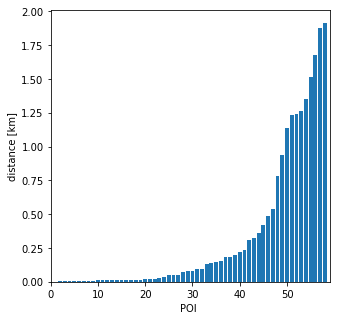
\includegraphics[]{images/distance.png}\\
%\caption{\label{fig:distance}This is a figure caption.}
\end{figure}
Looking at the distance distribution we note that most of the POIs are actually near to the Google Maps coordinates, while for few POIs this is not true. The main reason for this is the inherent unprecision that arise when wedefine a POI which occupies a big surface with coordinates that refer to a specific point. For example the surface of the airport of Nice is quite big and different services can locate it in different points of his surface. In the case of the airport, the distance is actually 500 meters. This means that if it is true that most of the POIs are under 500 meters, we can't use this as a threshold because we would leave out a large part of the correct POIs.

At the end of our POI linking process we have 58 POIs that will be matched with the artists.

\section{Interlinking and enriching Artists}
\subsection{Problem description}
DBpedia contains Artists and their works in a disorganized way.
This consist a huge limit because we do not trust the data that we have in DBpedia. Even the simpler operations, such as finding all artists and all songs are extremely difficult due to the non-strict ontology of DBpedia. In order to have some order, we use DOREMUS, which contains trusted informations about artists and songs in a strict ontology.

\subsection{Datasets: DOREMUS, DBpedia, Wikidata}
\subsubsection{DOREMUS}
DOREMUS is a semantic dataset that aims to a fine description of musical works in the fields of traditional and classical music: related musical or creation events, relations to authors, cultural background, interpretations, social functions, etc.
With DOREMUS we can have absolute trust in the data regarding artists, and we can then found corresponding artists in DBpedia with a custom linking process.

Retrieving all artists from DOREMUS is extremely easy, in fact we just need to ask for the Persons in the datasets. Then from these we filter persons that actually created at least a work.

\subsubsection{DBpedia}
Unfortunately DBpedia does not have a strict definition of a musical Artist. This means that retrieving artists from DBpedia is not trivial. What we do it to get all Persons, which are quite a lot. Most of them are not artists, and we filter them later.

todo: lorenzo


\subsubsection{Wikidata}
If Wikidata was extremely reliable for the POIs, it is not that strict about musical artists, in fact we need to get all persons and then filter them in some way, looking at classes that are related to music.

\subsection{Entity Linking process (+ ElasticSearch)}
Here we do the same thing that we did with POIs, we need to extract interesting properties from our entities and then use them to find the correct matches. 
With POIs we had one hundred entities from DBpedia, and we could do all operations locally. Here we would like to do the same, but we are dealing with millions of persons, and retrieving them and doing all operations locally is not feasible. For each artist in DOREMUS, we would compare his label with the label of millions of persons, and in Doremus we have thousands of artists.

In order to speedup operations, we use a dump of DBpedia indexed on ElasticSearch. This allow us to perform all the comparison in a fraction of time thanks to the use of indexes.

todo: Lorenzo


\subsubsection{Properties}
\subsubsection{Transformations}
\subsubsection{Similarity measures}
\subsubsection{Aggregations}
\subsubsection{Filtering}
\subsection{Evaluation}
The evaluation of the found links is done by comparing them with those provided by ISNI. ISNI is the ISO certified global standard number for identifying the millions of contributors to creative works. By achieving these goals the ISNI will act as a bridge identifier across multiple domains and become a critical component in Linked Data and Semantic Web applications.

ISNI matches are made by persons in the editorial world, so we can consider them as a ground truth that can be trusted. By comparing our matches we want to see if our performances are acceptable and if we can discover new links between ISNI numbers and DBpedia.

\begin{figure}
\centering
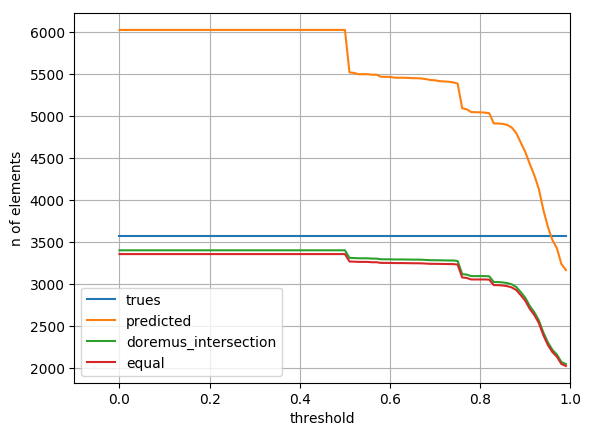
\includegraphics[]{images/counts_artists.png}\\
%\caption{\label{fig:distance}This is a figure caption.}
\end{figure}

Since the matching confidence vary with the threshold, we can plot all the important counts and metrics respect to the threshold used.

In the figure above there are all the counts of the important sets that describe our matching.
Trues indicates the number of doremus entities matched by ISNI, they are ~3500 and of course they are independent from the threshold.
Predicted indicates the number of doremus entities matched by us, the number vary with the confidence, there are different drops that corresponds to crucial thresholds defined by our matching algorithm. The most important thing is that their number goes from ~3000 to ~6000, this indicates that we are matching way more entities than ISNI.
Doremus intersection represents the number of entities that are matched from both ISNI and us. This shows us that there is a part of the doremus entities that ISNI matches and that we are not able to match.
Now, the following sets are all calculated from the intersection set, in fact we cannot compare the matching performances using entities that are not present in both sets.
Equal show the number of correct matches, we see that this basically overlap with the intersection set, meaning that ISNI and our algorithm match a doremus entity with the same DBpedia entity. Since ISNI matches have a professional validity, this means that we can have a great confidence in the matches produced by our algorithm.

Since equal and doremus intersection are not exactly the same, it means that either our algorithm or ISNI are doing a wrong match. Looking more closely we saw that in some cases ISNI matches were wrong, especially in corner cases, where there were two persons with the same name.
This corner cases can fool also a professionist, and this is the reason why in our algorithm we embedded the comparison of birthdate and deathdate in DBpedia with those present in Doremus. This allowed us to disambiguate between different persons with the same name. In other cases this was not enough, there are persons with the same name and birth/death dates, or whose dates are not available, that can be correctly classified looking at other fields, such as their profession.


\begin{figure}
\centering
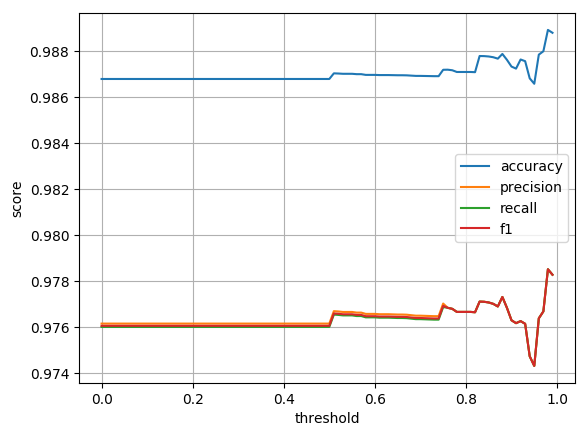
\includegraphics[]{images/metrics_artists.png}\\
%\caption{\label{fig:distance}This is a figure caption.}
\end{figure}
Looking at the usual metrics, we see that they are extremely high for this kind of match. This means that we are doing an almost perfect match.

We can state that the proposed method based on combinations of labels, classes and dates is able to match almost perfectly the artists of the two datasets. Moreover, we are able to find 2000 artists that at the time of writing are not present in the ISNI register.

\section{Path finder}
\subsection{Problem description}
Once we have a direct mapping between entities that comes from specialized datasets and DBpedia, we actually need to link POIs and Artists.
The problem of finding relations between entities in DBpedia has already been approached and solved in the past, especially from Relfinder. The whole problem can be solved by writing a single query that finds a path of a given depth between two resources. This approach works well when datasets are relatively small or the two entities are two concepts that are semantically close. Instead, in our case we have concepts that are absolutely far from each other, which implicates an high depth of an eventual path, and most importantly, we need to match hundreds of POIs with thousands of artists, This makes means that at the end the whole process will be repeated 25.000 times.
\subsection{Related work (Relfinder)}
The path finding problem has already been solved in the past with Relfinder: a tool that is able to find all paths with a specified depth between two entities. 
In fact, when we think at linking two entities, we need to set the position of the middle node and the number of middle nodes.

$$a-->b-->c-->d-->e=m$$
$$a-->b-->c-->d=m<--e$$
$$a-->b<--c=m-->d-->e$$

These are all different paths that links two entities 'a' and 'e'. In the simpler case, the arrows goes in one direction. In the second case they change direction one time.In the third case they change two times.
Relfinder manages to solve the problem by making different query that cover all possible combinations of the path specified above. As a constraint, in Relfinder the direction cannot change more than two times. There are still a huge amount of queries that explodes when the depth starts to be deep.
Here we intend as a deep depth a depth greater than 4, in fact this is like a magic threshold. 
Moreover, when we use Relfinder and set a greater depth we incur in two problems: 
\begin{enumerate}
\item The number of queries explodes because we need to consider all possible combinations
\item The time required by a single query explodes too, most of the times we cannot even do a query between two entities in a short time.
\end{enumerate}
In order to succeed we need to solve those two problem and we need to create a fast implementation, because at the end we will need to do 100.000 queries. 
\subsection{Proposed approach}
The problem is that DBpedia is small world and its average degree is 4.3, this means that on average we can reach every entity in at most 4-5 hops. Unfortunately our problem does not make part of that average, and many times we need 5-6 hops to connect two entities. The problem is that when we make a query that looks for paths with depth 6 we are basically querying the whole DBpedia, which at the time of writing is composed of 8.8 billion triples.
It is our belief that a query that tries to find a path between two entities, is converted by the SPARQL engine in what we can compare to a join for each hop. This, with the small world characteristic of DBpedia means that we are doing huge joins for each query.
Another way to visualize the query is a Breath First Search that starts from the source entity, and it expands hop after hop until the specified depth is reached. In this way is even more easy to see why we and up by querying billions of triples.
A common improvement of BFS is the two-way BFS, where the same algorithm is applied both at the source and the destination. In this way we can see that we can reach the same middle node by querying a way smaller portion of the graph.
Then, looking by hand at paths, we have seen that usually one direction inversion cover most of the cases, by limiting this we are actually simplifying a lot our problem. The, we have seen that for artists and POIs, the connection is most of the times the result of a common node. This means that the direction must change at least one time. We reduced all the different cases to one. In fact what we do is to make two separate queries with depth  from the source and from the destination. These queries return the list of all half-paths. We make a set of the involved nodes and then we intersect the two sets, in order to find the common nodes. At this point we operate joins that create full paths. The whole matching of POIs and Artists,100.000 combinations, requires only some hours against the weeks that would take relfinder.
\subsection{Selection Algorithm}
Now that we have all our path, we need to find the best ones, those that shows interesting links between POIs and Artists.
todo: lorenzo
\section{REST API}
The paths between a POI and the linked artists are exposed by a REST API that runs on Flask. Their extensible framework allows to develop several components requiring minimum boilerplate.
The main endpoint is the one that exposes the tracks and the paths related to a specific geoposition.
The whole process can be summarized in:
\begin{enumerate}
\item Take user position
\item Calculate nearest POIs and assign weights, from these create a univoque playlist name.
\item Select the tracks for each artist linked with the poi.
\item Select for each artist a compatible number of tracks to put in the playlist.
\item Create a playlist if it does not exist and add previously selected tracks.
\item Attach to each track the path between the poi and the track's artist.
\item Return the playlist ID and the track-path mappings as a JSON.
\end{enumerate}
\subsection{Spotify API usage}
Spotify provides a public API that allows to perform all the operations that can be done using the Spotify application. These comprend artist and tracks search, CRUD operations on user playlists and the listening of the tracks' preview.
\subsubsection{Authentication}
Since the end user listen to a spotify loaded dynamically by the application, there is no need for a client authentication. This is perfect because it allows to any user to use our application. Regarding the server, At startup it is performed a token based authentication, where the server get possess of a private token used to perform all CRUD operations on the playlist catalogue.
\subsubsection{Playlist}
A playlist can be dynamically created. At creation time, it is required to give a name to the playlist, and the whole playlist object, containing the univoque playlist ID is returned. Later it is possible to access to the playlist either using the playlist ID or using the playlist name. The playlist name is univoque inside the application by construction, while the playlist ID is univoque for all Spotify playlists.
\subsubsection{Artist}
An artist can be searched by name, this part is the most critical one because Spotify does not provide any automatic artist matching using the api. This means that specifying the full name of the artist is essential for the success of this operation.
This is done by using the Doremus person label property, which consists of name and surname of the artist. It is interesting to note that from this point of view DBpedia is not reliable because the person label can contains adjectives used for the disambiguation of this one, such as 'Composer'. If this adjectives are passed to the Spotify search endpoint, no artist is returned.
When a request is done, Spotify returns a list of matching artists. Each artist object contains different informations, among them the most useful are the genres and the popularity. 
In order to limit outliers, not only we select the most popular artist, but we check that it has at least 10 popular songs, where popular songs are special songs selected by spotify. The popularity metric algorithm is not public, but it is based on the playcounts and the recentness of the track.
Here we use the popularity as a criteria to select the correct artist, in fact we take always the most popular. The use of the genre specification would be interesting for an ulterior enhancement.
\subsubsection{Tracks}
Among all properties that caracterize a track, we only need the ID and the name.

\subsection{Playlist Endpoint}
\subsubsection{Nearest POIs selection algorithm}
In order to match a position with a list of POIs, the following algorithm is followed:
\begin{enumerate}
\item Calculate distance from the each POI to the user position. Since we are using coordinates, the distance is calculated using the haversine distance, which is very accurate and fast.
\item Add to the list the nearest POI, regardless of the distance.
\item Add the remaining two nearest POIs if their distance is inferior of 1 km.
\item For each element in the list, add 10 meters to the distance and then take the log2. By adding 10 meters we are adding a bias to all our distances, in this way positions too near to us are not over-weighted respect far distances. Then, the log2 squashes distances until 1 km to a restricted range of values.
\item Calculate repartition weights using the following equation:
$$w_i = \Bigg \lfloor 10 \dfrac{\dfrac{1}{\log_2 (d_i + 10)}}{\sum \dfrac{1}{\log_2 (d_i + 10)} } \Bigg \rceil$$
In this way we obtain normalized weights from 0 to 10 that are inversely proportional to the log base 2 of the distance. 
\end{enumerate}
At this point we have a direct mapping between POIs weights and a position
\subsection{Artist' tracks selection algorithm}
For each artist there is a direct mapping with its tracks.
The problem is: given a playlist name, find the correct tracks.
The playlist name encodes the weights of each poi, and each weight express exactly the number of tracks that must be chosen for the POI associated.
Since each POI is linked to different artists, we need a way to select songs from them in a balanced way.
What we do is to cycle between all the artists to take each time the most important song that is not already present in the playlist. In this way we obtain different songs from different artists, and since the artist and songs are static, the tracks in the playlist will be always the same. In the future we think to add randomicity to the whole selection process.

\subsection{Response generation}
\begin{enumerate}
\item Generate playlist name as described before
\item Select tracks as described before
\item Create a playlist if it does not exist and add previously selected tracks.
\item Attach to each track the path between the poi and the track's artist.
\item Return the playlist ID and the track-path mappings as a JSON.
\end{enumerate}

\section{Mobile Web Application}
\subsubsection{Music Player}
The music player is implemented using the Spotify Play Button. This is a special iframe that loads a simplified Spotify player for a specified playlist. This solution is extremely convenient because it simply needs a plylist ID to run. Since the playlists are created server side and are recovered using the REST API, the whole process is very simple.
Unfortunately it is not possible to manipulate programmatically the iframe and this limit the whole user experience. As an improvement, we could build a custom player that still uses the Spotify API.
\subsection{Google Map API}
\subsubsection{POIs placement}
todo: Lorenzo

\subsubsection{Navigation}

\subsection{Relation visualization (and Path format)}
todo: Lorenzo
\section{Conclusion and Future Work}
Regarding the fact that is difficult to evaluate the performances of a recommender system, in fact a user may seem appropriate the link but not like the song, we are convinced of our results.
Regarding the first part: the interlinking, we can refer to the evaluation section of the two approaches. Regarding POIS, we see that we achieve a perfect POIs matching: matched POIS are 99\% correct, and their positioning is very accurate, comparable to Google Maps.

Regarding the Artist matching, we obtained a perfect match, in fact we have checked that our linker fails when the ISNI matches are wrong. Moreover, we have found 3000 entities with high confidence that are not matched by ISNI. So we think that this linker can definetly considered a success.

Pathfinding: we created a way that has never been publicated that is actually scalable. We think that having scalable solution for the relation finding is crucial for any project that aims to use heavily the huge knowledge graph that DBpedia is.

Moreover, we find a good use of an equation proposed in another paper. todo. cite




The high precision values (over 80% for top 5 results in

Table 1) obtained by the evaluated recommendations let us

claim that our approach is able to automatically identify

musicians semantically related to a given place of interest

(RQ1). The user studies also showed that, in our approach,

musicians evaluated as relevant tend to have relative high

numbers of paths in a POI’s semantic network for all the

proposed types of relations (i.e., city, date and category),

while these numbers are significantly lower for non-relevant

musicians. This evidences that our approach, which is based

on finding semantic paths between POIs and musicians, can

be used effectively to define and evaluate the semantic relat-
edness between such instances (RQ2). Moreover, we have

shown that users perceive music composed/performed by the

recommended musicians as well-suited for the POIs.

We note that the presented framework fully relies on the

data available in DBPedia repository – in order for a mu-
sician to be recommended by our approach, its record has

to be present in DBPedia. Admittedly, this is a limitation,

since less known musicians may not have DBPedia entries.

In the future, this could be addressed by using additional

Linked Data repositories.

An important next step in this research is adapting the

proposed framework to incorporate user preferences into the

recommendation process. As described in Section 3.1, this

can be achieved using the weights of relations between classes

and instances in the semantic network. We intend to ex-
plore personalization approaches that translate user’s pref-
erences into these weights.
It is also important to better explore and evaluate strate-
gies to initialize the importance weights of the relations and

classes in the semantic network. In this context, we will ex-
plore other approaches to define and measure the semantic

relatedness between concepts [13], and will adapt or extend

them for cases in which the concepts belong to different do-
mains.

Your introduction goes here! Some examples of commonly used commands and features are listed below, to help you get started.

If you have a question, please use the support box in the bottom right of the screen to get in touch. 

\section{Some \LaTeX{} Examples}
\label{sec:examples}

\subsection{Sections}

Use section and subsection commands to organize your document. \LaTeX{} handles all the formatting and numbering automatically. Use ref and label commands for cross-references.

\subsection{Tables and Figures}

Use the table and tabular commands for basic tables --- see Table~\ref{tab:widgets}, for example. You can upload a figure (JPEG, PNG or PDF) using the files menu. To include it in your document, use the includegraphics command as in the code for Figure~\ref{fig:frog} below.

% Commands to include a figure:
\begin{figure}
\centering

\includegraphics[width=0.5\textwidth]{images/frog.jpg}
\caption{\label{fig:frog}This is a figure caption.}
\end{figure}

\begin{table}
\centering
\begin{tabular}{l|r}
Item & Quantity \\\hline
Widgets & 42 \\
Gadgets & 13
\end{tabular}
\caption{\label{tab:widgets}An example table.}
\end{table}

\subsection{Mathematics}

\LaTeX{} is great at typesetting mathematics. Let $X_1, X_2, \ldots, X_n$ be a sequence of independent and identically distributed random variables with $\text{E}[X_i] = \mu$ and $\text{Var}[X_i] = \sigma^2 < \infty$, and let
$$S_n = \frac{X_1 + X_2 + \cdots + X_n}{n}
      = \frac{1}{n}\sum_{i}^{n} X_i$$
denote their mean. Then as $n$ approaches infinity, the random variables $\sqrt{n}(S_n - \mu)$ converge in distribution to a normal $\mathcal{N}(0, \sigma^2)$.

\subsection{Lists}

You can make lists with automatic numbering \dots

\begin{enumerate}
\item Like this,
\item and like this.
\end{enumerate}
\dots or bullet points \dots
\begin{itemize}
\item Like this,
\item and like this.
\end{itemize}

We hope you find write\LaTeX\ useful, and please let us know if you have any feedback using the help menu above.

\end{document}